% !TEX root = ../../numb3rs.tex
\newpage
\section{Season 3}
\subsection{301: Spree\label{301}}

In this episode, Crystal and her boyfriend Buck engage in a robbery and killer spree. Charlie uses pursuit curves to determine their next move.

%%%%%%%%%%
\temph{Pursuit Curves}
%%%%%%%%%%

In order to understand the route taken by the wanted couple and possibly predict their next move, Charlie realizes that he can use the theory of pursuit curves. Basically, a pursuit curve is the path described by an object $A$ when it is chasing an object $B$. For instance, think of a cat chasing a mouse. Object $A$ chases object $B$ in such a way that:
	\begin{enumerate}[(i)]
	\item $A$ always heads directly toward $B$.
	\item A's speed is proportional to B's speed. That is, if B goes faster/slower, then so does B. (We assume that A's speed is constant).
	\end{enumerate}
Our first activity will be to formalize the definition. \\

\fbox{\begin{minipage}{43em}
\begin{center} \large \dotuline{Activity 1}  \\ \end{center}
Suppose that the pursued (the mouse) moves along a curve $F=(f(t), g(t))$ and the pursuer (the cat) moves along a curve $G(t)=(a(t), b(t))$. Write equations to describe $(i)$ and $(ii)$ above.
\end{minipage}} \vspace{0.2cm}


\fbox{\begin{minipage}{43em}
\begin{center} \large \dotuline{Tangent}  \\ \end{center}
Leonardo da Vinci was the first one to study this problem when the pursued moved along a straight line. The general case was studied in 1732 by Pierre Bouguer (1698--1758), the French scientist who first attempted measuring the density of the Earth considering the deflection of a plumb line due to the attraction of a mountain.
	\begin{figure}[H]
	   \centering
	   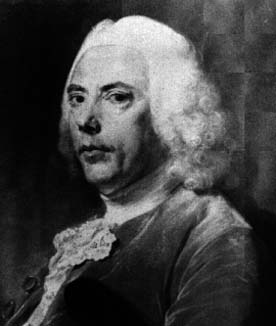
\includegraphics[width=0.2\textwidth]{season3/301/images/Bouguer.jpg} 
	\end{figure}
\end{minipage}} \vspace{0.2cm}

Let us not draw examples of these curves. Suppose you have three people, say $A$, $B$, and $C$, in three different corners of an equilateral triangle. Each person chases the person to his/her right. Let us draw the first step of of the curves described by each of these three people below.
	\begin{figure}[H]
	   \centering
	   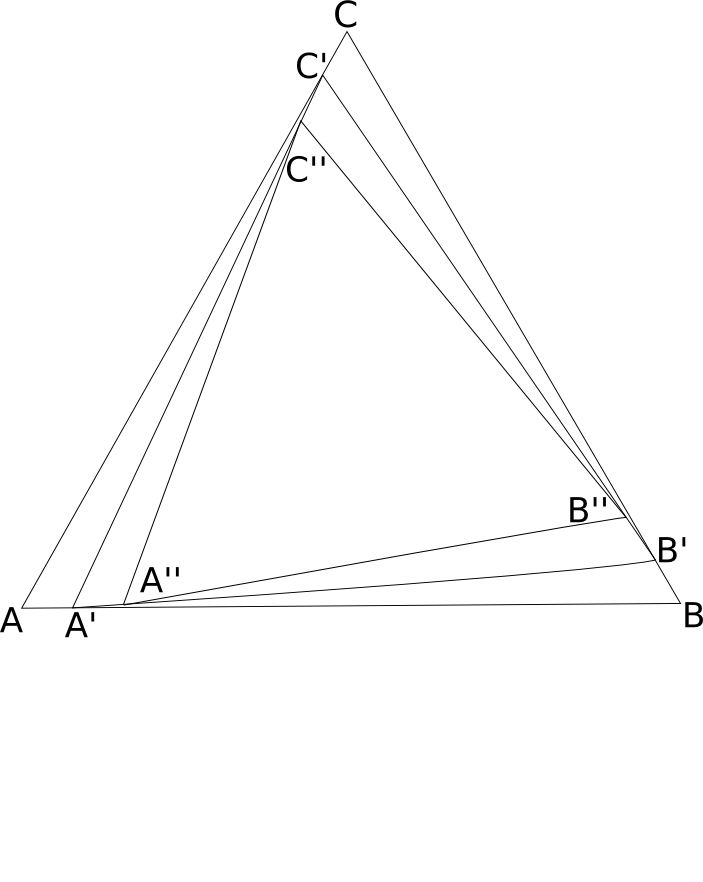
\includegraphics[width=0.4\textwidth]{season3/301/images/triangle1.png} 
	\end{figure}

After 1 second, $A$, $B$, and $C$ have moved to $A'$, $B'$, and $C'$, respectively. Furthermore, after two seconds, their new position is $A''$, $B''$, and $C''$. The points $A$, $A'$, $A''$,\dots belong to the pursuit curve of $A$ chasing $B$; the points $B$, $B'$, $B''$,\dots belong to the pursuit curve of $B$ chasing $C$; and the points $C$, $C'$, $C''$,\dots belong to the pursuit curve of $C$ chasing $A$. \\

The construction indicated above produces the beautiful drawing below, by John Sharp. Notice that all three curves forms spirals that converge to the center of the triangle
	\begin{figure}[H]
	   \centering
	   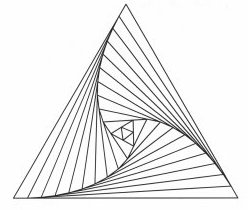
\includegraphics[width=0.4\textwidth]{season3/301/images/triangle2.jpg} 
	\end{figure}


\fbox{\begin{minipage}{43em}
\begin{center} \large \dotuline{Activity 2}  \\ \end{center}
\begin{enumerate}[1.]
\item Apply the construction in the case of a square. Describe the shape of the pursuit curves.
\item Argue that all in the case of an equilateral triangle and the square, all pursuit curves meet at one point. What is this point? What happens to other polygons?
\item It can be shown that for any triangle, the pursuit curves constructed above intersect in a point known as Brocard point. Argue that a general triangle has exactly two Brocard points (if the triangle is equilateral, these points are the same).
\item[4*.] Denote the two Brocard points by $P$ and $Q$. Show that the angles  $\angle PAB$ = $\angle PBC = \angle PCA = \angle QCB = \angle QBA = \angle QAC$.
\end{enumerate}
\end{minipage}} \vspace{0.2cm}

%%%%%%%%%%
\temph{Computing Pursuit Curves}
%%%%%%%%%%

Now we focus on computing pursuit curves. We denote by $M$ the curve describer by the pursued object (mouse), which we assumed known, and by $C$ the curve described by the pursuer (cat). Notice that $i$ above implies that
	\[
	\dfrac{\vec{M} - \vec{C}}{\left| \vec{M} - \vec{C}\right|} \cdot \dfrac{\vec{C}'}{\left|\vec{C}'\right|} = 1
	\]
since the cat is always looking directly at the mouse (that is, the pursued is in the tangent vector of the pursuer). This equation appears in many shots of the episode. Furthermore, without loss of generality we can assume that  
	\[
	\vec{C}' \cdot \vec{C}' = \left|\vec{C}'\right|^2=1
	\]
since we assume that the cat's velocity is constant. These yield a system of \emph{differential equations} that can be used to find (or approximate) the coordinates of the pursuit curve. \\

\fbox{\begin{minipage}{43em}
\begin{center} \large \dotuline{Activity 3}  \\ \end{center}
\begin{enumerate}[1.]
\item[1*.] Use the equations above to deduce a system of two differential equations involving the components of the pursuit curve $C$ in the plane.
\item[2.] Alternatively, consider the following procedure:
	\begin{enumerate}[a.]
	\item Denote by $v_m$ and $v_c$ the velocity of the mouse and cat, respectively. $(ii)$ in the definition gives that $v_c = kv_c$. Use this to express the tangent (unit) vector of C, TC in terms of $v_c$ and $v_m$.
	\item Using $(i)$ above, note that $T_C$ in terms of the vector $\vec{M} - \vec{C}$.
	\item Use 1 and 2 above to deduce 
		\[
		\vec{v}_c = k \left|\vec{v}_m\right| \, \dfrac{\vec{M} - \vec{C}}{\left| \vec{M} - \vec{C} \right|}
		\]
 	and use that expression to obtain the system in $(i)$.
	\end{enumerate}
\end{enumerate}
\end{minipage}} \vspace{0.2cm}

In the previous activity we assumed that the pursued curve was known. Notice that this is slightly different from the pursuit curves of Activity 2, since there are more individuals involved. For instance, consider the \emph{four bugs problem}, where there are 4 bugs placed each at one corner of a square. Each bug chases the bug immediately to its right at constant speed. In the next activity we describe the pursuit curves (with equations).

\fbox{\begin{minipage}{43em}
\begin{center} \large \dotuline{Activity 4}  \\ \end{center}
\begin{enumerate}[a.]
\item Draw a picture of a square on the plan and place a bug in each of the corners. We suggest the coordinates $(1,0)$, $(0,-1)$, $(-1,0)$, and $(0,1)$.
\item Let $\mathbf{P} = (x,y)$ and $\mathbf{Q} = (u,v)$ be the pursuit curve of two bugs that are in consecutive corners, with the bug along $\mathbf{P}$ chasing the bug along $\mathbf{Q}$, and $\mathbf{P}$ starting at $(1,0)$. Deduce that $x = v$ and $y = -u$.
\item Use b. to show to obtain the vector $\mathbf{P} - \mathbf{Q}$ in terms of $x$ and $y$.
\item If $x = x(t)$ and $y = y(t)$ are parameterizations of $\mathbf{P}$. Since the bug along $\mathbf{P}'$ is heading directly at the bug along $\mathbf{Q}$, the direction of $\mathbf{P}$'s movement are also given by $(x'(t),y'(t))$. If this is the case, deduce that $x(t) = e^{-t}\cos t$ and $y(t)=e^{-t}\sin t$.
\item What is the distance that each bug travels?
\end{enumerate}
\end{minipage}} \vspace{0.2cm}


\fbox{\begin{minipage}{43em}
\begin{center} \large \dotuline{Tangent}  \\ \end{center}
The pursuit curves are sketched below. This is the same picture we would have obtained by the construction described before Activity 2. Notice that it takes an infinite amount of time for the bugs to reach the origin. Can you see this from the equations?
	\begin{figure}[H]
	   \centering
	   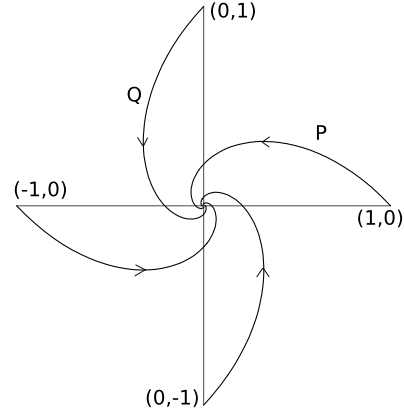
\includegraphics[width=0.3\textwidth]{season3/301/images/4bs.png} 
	\end{figure}
\end{minipage}} \vspace{0.2cm}

%%%%%%%%%%
\temph{Sketching Pursuit Curves}
%%%%%%%%%%

The system of differential equations obtained in the previous activity is generally generally very hard to solve. On the other hand, one can easily plot the pursuit curve of certain scenarios. \\

\fbox{\begin{minipage}{43em}
\begin{center} \large \dotuline{Activity 1}  \\ \end{center}
Suppose a mouse moves along a circle of radius $r$. Suppose there is a cat at the center of the circle.
\begin{enumerate}[a.]
\item Sketch the pursuit curve described by the mouse chasing the cat. Is it possible for the cat to catch the mouse?
\item What if the cat is at a distance 2r from the center of the circle?
\end{enumerate}
\end{minipage}} \vspace{0.2cm}

